% !TeX spellcheck = <none>
\documentclass[a4paper]{article}
\usepackage[utf8]{inputenc}
\usepackage{float}
\usepackage{geometry}
\usepackage{graphicx}
\usepackage[bookmarks=true]{hyperref}
\geometry{left=1.0cm, right=1.0cm, top=1.5cm, bottom=1.5cm}
\usepackage{amsmath}
\usepackage{amsfonts}
\usepackage{mathrsfs}
\usepackage{caption}
\usepackage{indentfirst}
\usepackage{float}
\usepackage[scheme=plain, UTF8]{ctex}
\usepackage{bm}
\linespread{1.0}
\newcommand{\sep}{\noalign{\vskip6pt}}
\usepackage{chemarr}
\usepackage{fontspec}
\usepackage{enumerate}
\usepackage{setspace}
\usepackage{array}
\usepackage{booktabs} %调整表格线与上下内容的间隔
\usepackage{multirow}
\usepackage{subfigure}
\renewcommand\refname{参考文献}
\linespread{1.0}
\everymath{\displaystyle}
\begin{document}
	\begin{center}
		\begin{LARGE}
			《毛泽东思想和中国特色社会主义理论习题概论》实践课
		\end{LARGE}
	\end{center}
	\vskip10pt
	\begin{center}
		\begin{Huge}
			\centering
			\textbf{社会调查报告}
		\end{Huge}
		\vskip60pt
		\begin{Large}
			\begin{tabular}{lcr}
				题目 & 对“二次元”及其衍生品Cosplay的认知态度问题\\
				\specialrule{0em}{40pt}{40pt}
				姓名 & 徐亦捷\\
				& 徐润奇\\
				& 周润东\\
				& 曾沛然\\
				\specialrule{0em}{40pt}{40pt}
				学号 & 201883100068\\
				& 201883100067\\
				& 201883100023\\
				& 201883100070\\
				\specialrule{0em}{40pt}{40pt}
				专业 & 数学与应用数学
			\end{tabular}
		\end{Large}
		\vskip200pt
		二〇二一年六月十四日
	\end{center}
	\clearpage
	\tableofcontents
	\clearpage
	\section{背景部分}
	\subsection{什么是二次元}
	若从客观科学的角度来说,二次元就是二维的意思,英文为“Two dimensions”。与我们平时立体的三维空间相对比,“二次元”指的是二维的平面,进而引申出通过平面所呈现的动漫影视、漫画、游戏等等。这样创造出的虚拟世界,被称为是“二次元”。二次元通常也是指幻想中的世界,类似地,“三次元”指我们的现实世界。当代我国“二次元”发展十分快速,以至于短短十几年间,不同“二次元”用户竟能产生多道代沟。
	\subsection{什么是Cosplay}
	“Cosplay”是英文Costume Play的简写,日文为コスプレ,中文常将其翻译为“扮装游戏”。指利用服装、饰品、道具以及化妆来扮演动漫、游戏中以及古代人物的角色。玩COSPLAY的人则一般被称为Cosplayer,或Coser。\\
	\begin{figure}[H]
		\centering
		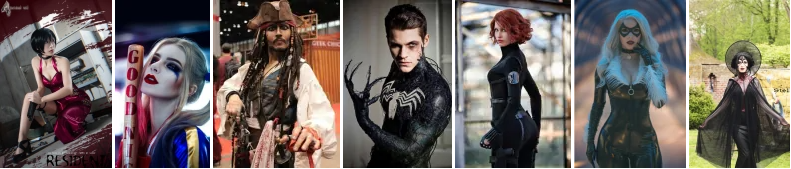
\includegraphics[width=0.5\linewidth]{figures/1}
		\caption*{一些常见的Cosplay角色图}
	\end{figure}
	
	经过长时间的发展与探究,如今的扮装已经演变得相当完善与发达,不仅可以扮演人形动漫角色,而且更可以扮演漫画和游戏中任何的东西,例如动物、机械人,没有任何限制。作为“二次元”的附属文化,Cosplay在当今社会已经越发成为一种青少年文化娱乐的主流。
	\begin{figure}[H]
		\centering
		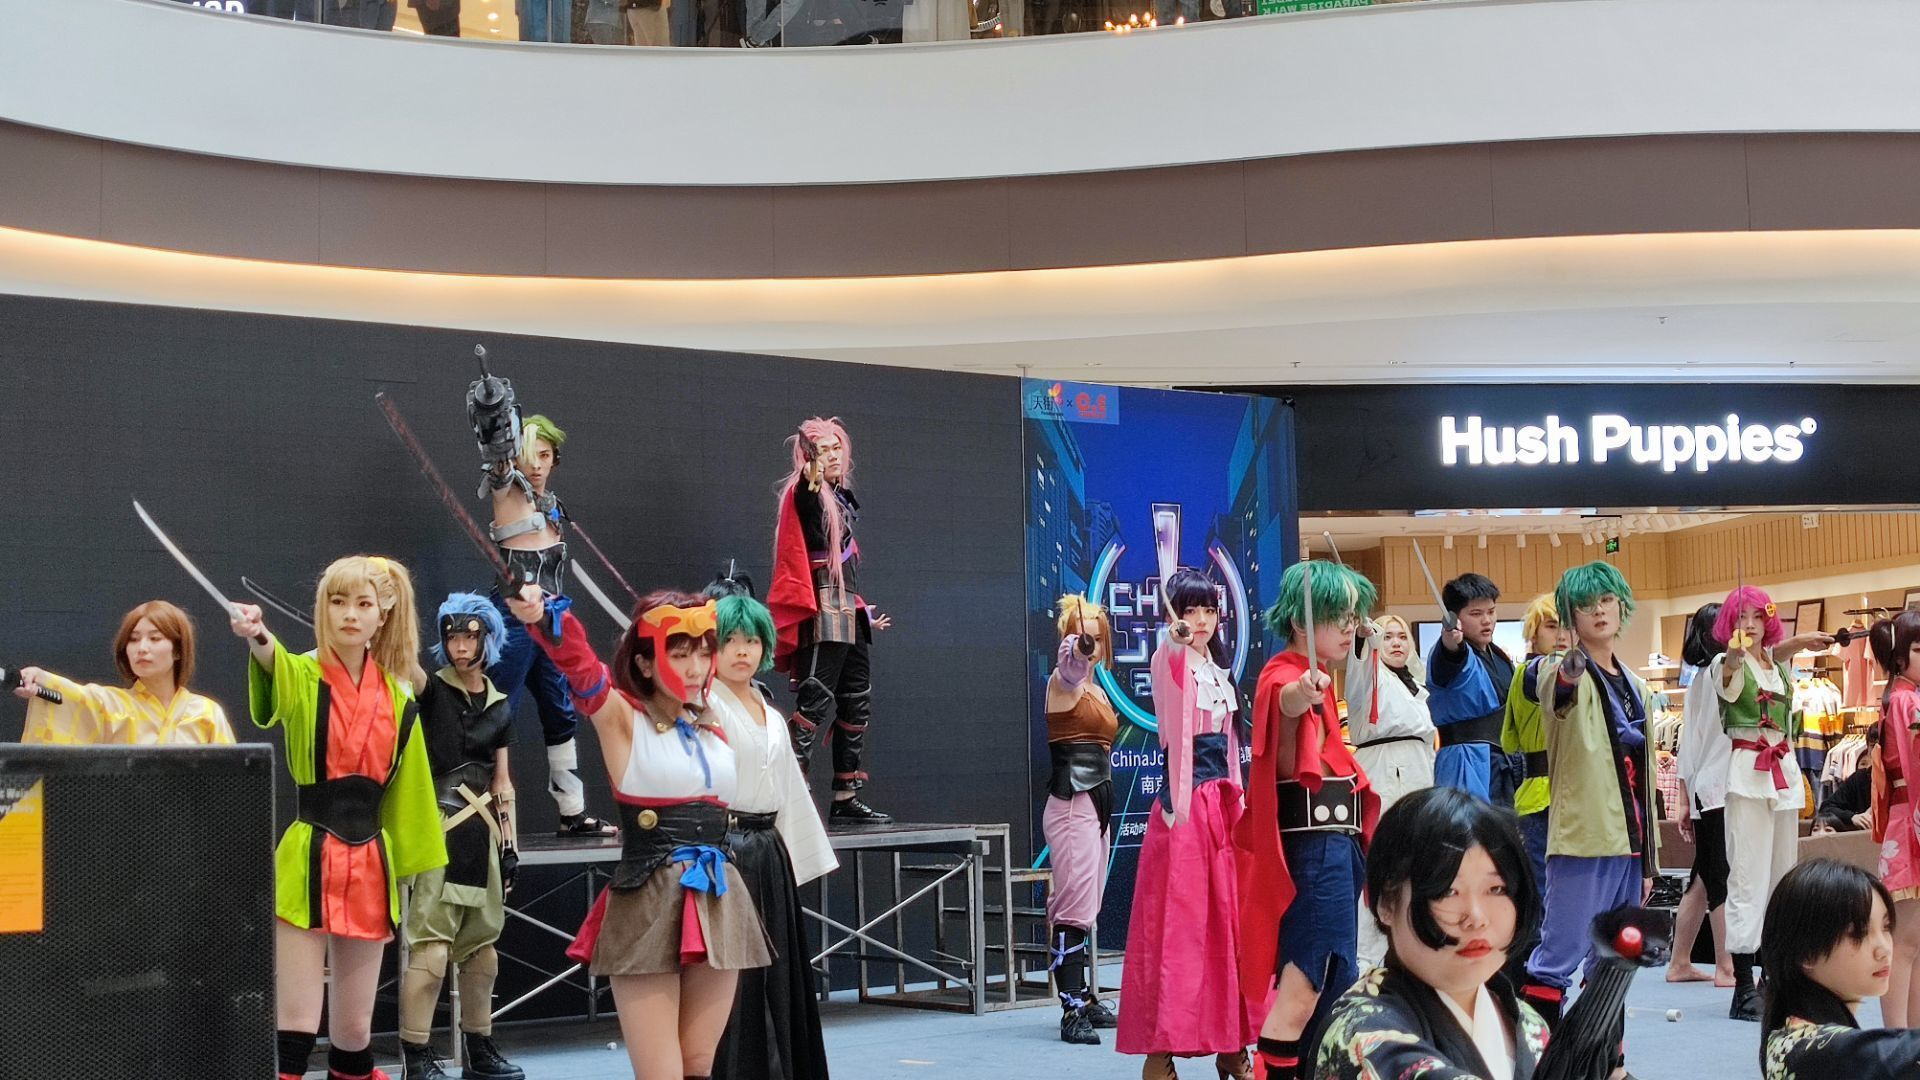
\includegraphics[width=0.5\linewidth]{figures/9}
		\caption*{游戏《原神》中角色的Cosplay}
	\end{figure}
	
	\subsection{Cosplay的乱象}
	首先在百度搜索Cosplay,自动跳出的不堪入目的“推荐搜索”就能很好的反映了这个圈子与文化所存在的问题。\\
	\begin{figure}[H]
		\centering
		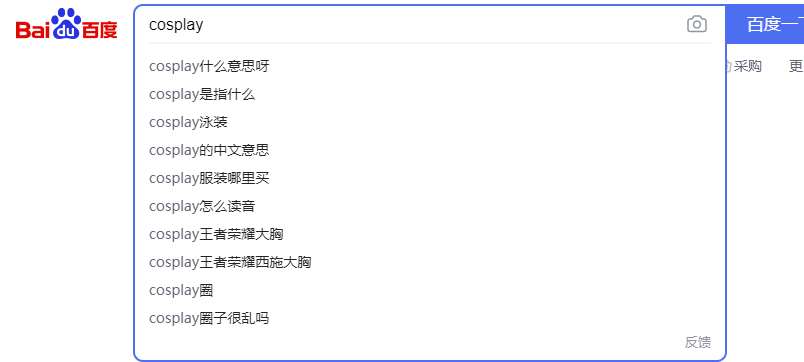
\includegraphics[width=0.5\linewidth]{figures/2}
		\caption*{百度搜索“Cosplay”的相关推荐}
	\end{figure}
	
	同时在我们的调查报告中,大家对于“二次元”和Cosplay的评分差异,对于身边人对于Cosplay的看法,也可以说明部分问题。在四张图表中,分数为1-5,越高则代表接受程度越高/可能性越大。\\
	
	\begin{figure}[htbp]
		\centering
		\subfigure[对于二次元的接受程度]{
			\begin{minipage}[t]{0.25\linewidth}
				\centering
				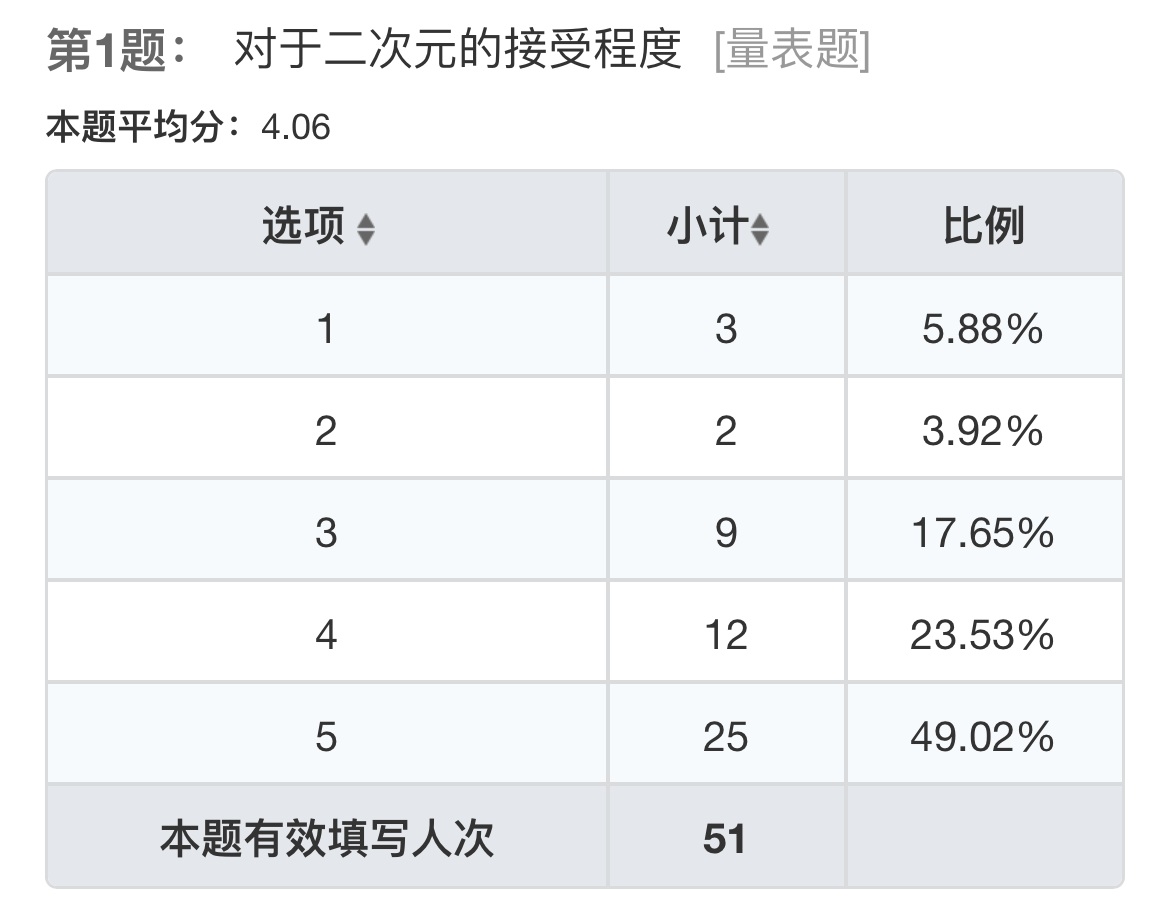
\includegraphics[width=1.5in]{figures/2x2_1}
				%\caption{fig1}
			\end{minipage}%
		}%
		\subfigure[对于Cosplay的接受程度]{
			\begin{minipage}[t]{0.25\linewidth}
				\centering
				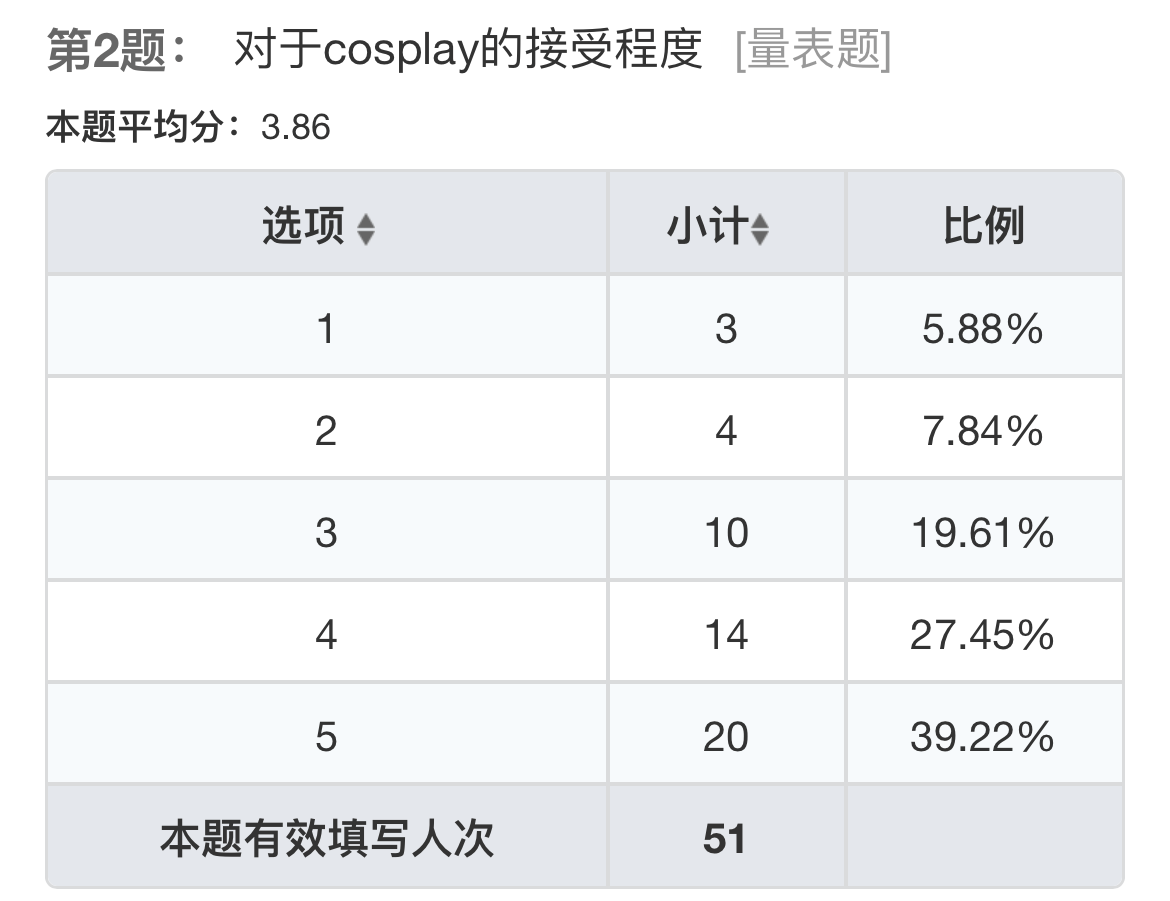
\includegraphics[width=1.5in]{figures/2x2_2}
				%\caption{fig2}
			\end{minipage}%
		}%
		\subfigure[自己参与的可能性]{
			\begin{minipage}[t]{0.25\linewidth}
				\centering
				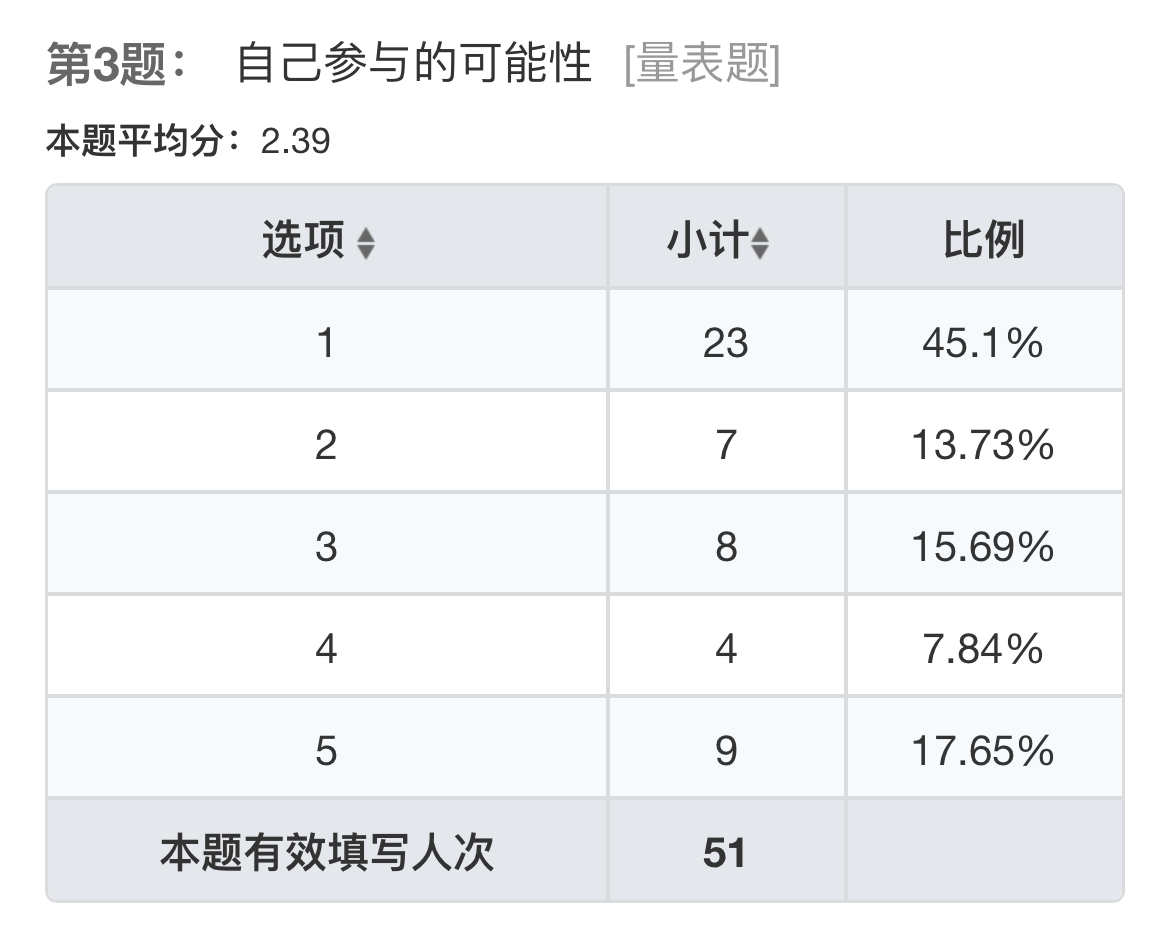
\includegraphics[width=1.5in]{figures/2x2_3}
				%\caption{fig2}
			\end{minipage}
		}%
		\subfigure[自己身边的人如何看待]{
			\begin{minipage}[t]{0.25\linewidth}
				\centering
				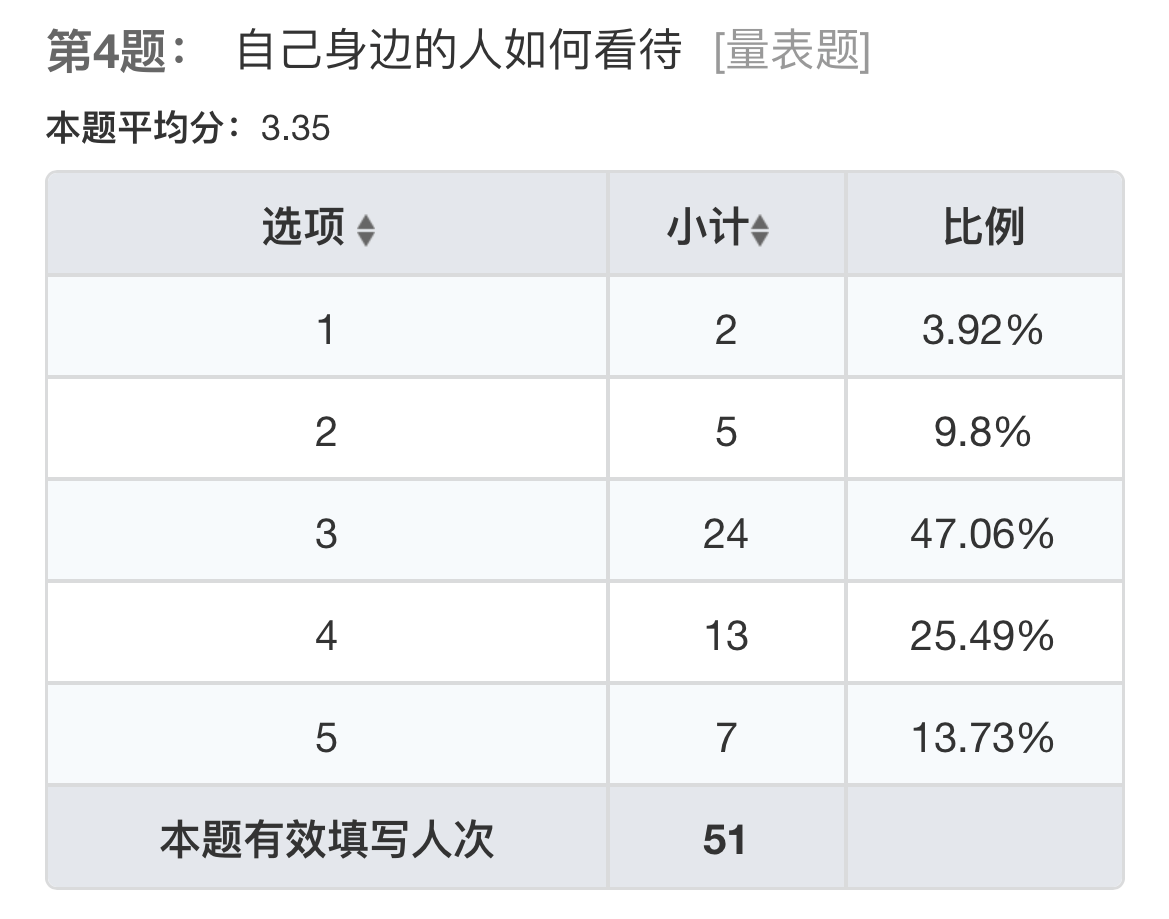
\includegraphics[width=1.5in]{figures/2x2_4}
				%\caption{fig2}
			\end{minipage}
		}%
	\end{figure}
	
	可以看到,接受调查的大多数年轻人对于Cosplay接受度都较高,然而自己参与的可能性却与之相反。同时,身边的人对Cosplay的态度亦低于自己对于Cosplay的接受度,这也部分反映了Cosplay圈目前的部分乱象给人的负面印象。\\
	
	本文将综合罗列几个Cosplay圈较为常见的乱象。
	\subsubsection{尺度过于暴露}
	根据Coser的定义,只要是进行Cosplay的人员都可以被视为Coser。因此,将动漫角色还原得较好的人员也在该圈子里有着较高的地位与知名度,从而容易进行流量变现以获利。然而,大量所谓的Coser在微博等平台上希望通过发布一些穿着极其暴露的大尺度图片而不是认真还原动漫角色的手段成名,用低俗的方式吸引眼球的同时也不尊重原著角色的造型。Cosplay的初衷是出于对自己喜欢的动漫角色热爱,去扮演自己的喜欢角色。而现在这些所谓的Coser其实只是以Cosplay为噱头卖肉从而吸引打赏,赚取金钱,从而带动了更多的不良行为,也给这个圈子带来了污浊的风气。
	
	\subsubsection{Cos圈中的“援助交际”}
	前些年有一条新闻爆火:“Cos圈援交”\cite{ref1}。 援助交际(えんじょこうさい),简称 “援交”,是一个源自日本的名词。根据赵军的论文指出\cite{ref2},援交最初指少女为获得金钱而答应与男士约会,后逐渐演化为学生“卖春”的代名词。Chau-kiu Cheung等人亦指出\cite{ref3},援助交际不一定有性交行为发生,也可能只是暧昧行为。援助交际具有参与人群广泛化、低龄化和参与途径多样化的特点。未成年人通常是因为金钱需求或性需求的驱使而选择进行援助交际,也有部分人是出于寻求自我价值与自我掌控权的考虑而进行援助交际。
	
	在本则新闻中的二次元Cos零花钱援交,顾名思义,就是Coser为赚取更多零花钱与他人做援助交际的行为。这些人喜欢玩Cosplay,单有些爱好太烧钱,尚无收入的人仅仅凭父母给的零花钱无法支付起置装费、道具费,因此有一些Coser会为了维持自己的爱好而去赚取一些额外的零花钱,援交便是其中一种方式。\\
	
	此外,部分未成年和或者刚成年的少女为了获得Cosplay道具,摄影等条件需要满足的金钱,竟然拉了个所谓“Cosplay零花钱”的群,通过线人“介绍客户”,以有偿陪同逛街和过夜的方式赚取金钱来满足自己Cosplay的需求。\\
	\begin{figure}[H]
		\centering
		\begin{minipage}[t]{0.48\textwidth}
			\centering
			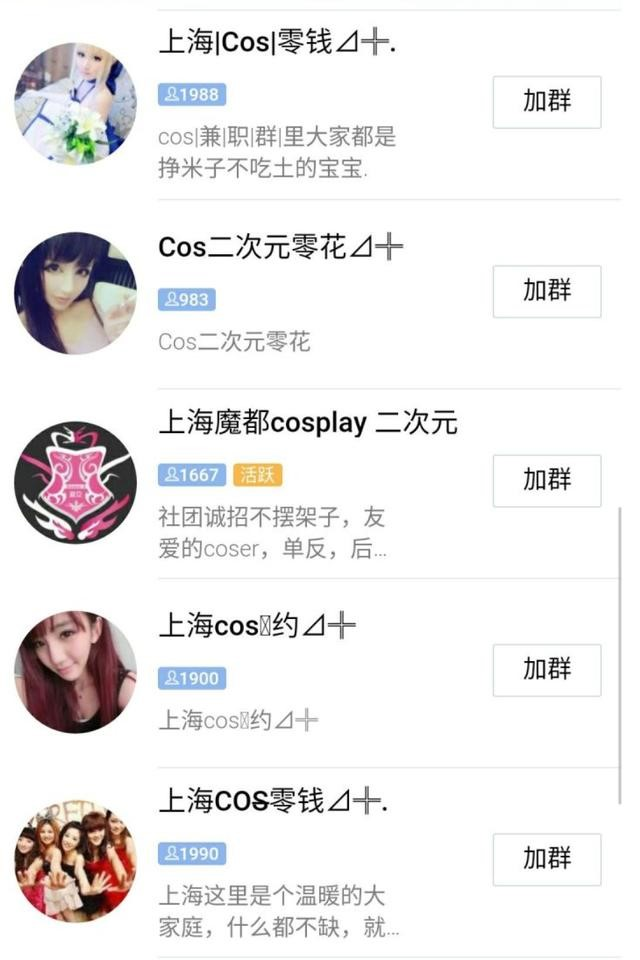
\includegraphics[height=8cm]{figures/3}
			\caption*{搜索含有“Cos”的QQ群结果}
		\end{minipage}
		\begin{minipage}[t]{0.48\textwidth}
			\centering
			
\includegraphics[height=8cm]{figures/4}
			\caption*{一个拉客援交的少女对话}
		\end{minipage}
	\end{figure}
	
	Cosplay的群体大多是大学生或者刚刚步入社会的年轻人,这个年龄的年轻人更有可能虚荣心强,且较懵懂,部分年轻人因为受教育水平低或其他原因,为了钱可以出卖自己的身体。不仅如此,还有一些Cos圈的摄影师以拍私房照为由,欺骗刚入行Coser从事服务,从而一步步走向不归路,败坏了整个行业的风气,甚至形成了一种不可描述的潜规则。\\
	
	需要指出,在我国的法律体系下,“援交”与卖淫无异,同样属于违法行为。部分Cosplay爱好者为了爱好竟堕落到如此底部,令人叹惋。
	
	\subsubsection{Cosplay圈不成体系,行业规范和制度不成熟}
	中国的二次元动漫产业完全没有形成一个健康的盈利生态,而漫展的存活也只能靠奇装异服甚至暴露的穿着打扮Cosplay来吸引外界人士。同时,与公司签约的Coser频频爆出各种没有职业道德的新闻:这些大牌签约Coser仗着自己粉丝多,缺乏契约精神,不履行自己的义务,随意耍大牌,不参加公司的活动。若公司要解约,他们就向粉丝哭诉以博得同情,以期用舆论给公司造成负面影响。这种行为败坏整个行业的风气。久而久之形成恶性循环,使得整个圈子的管理与运作陷入一片混乱,极大地阻碍了该行业在中国的健康运行与发展。
	
	\clearpage
	\section{讨论部分}
	\subsection{关于“性感”的讨论}
	任何文明的发展中,社会群体为了控制人口等目的,必然会有各种形式上的性压制,如在伊斯兰文明中,根据《古兰经》要求,妇女必须遮盖头部、颈部和胸部以保护其荣誉和尊严。更甚者在部分伊斯兰地区,女性被要求穿着布卡罩袍。布卡罩袍是一种具有穆斯林原教旨色彩的女性服装,主要为长袍、头巾加面罩,把女性从头到脚严严实实地包裹起来,只露出眼睛。而基督教中,《哥林多前书》中提到,圣保罗说到:“你们岂不知,不义的人不能承受神的么?不要自欺,无论是淫乱的、拜偶像的、奸淫的、作娈童的、亲男色的、偷窃的、贪婪的、醉酒的、辱骂的、勒索的,都不能承受神的国。你们中间也有人从前是这样,但如今你们奉主耶稣基督的名,并借着我们神的灵,已经洗净,成圣称义了。”而在我们中国的这片广袤的大地上,更是有“谈性色变”的传统。著名文学家鲁迅也因此痛批“一见到短袖子,立刻想到白胳膊,立刻想到全裸体,立刻想到生殖器...中国人的想象惟在这一层能够如此跃进。”\\
	
	在这里讨论这种性压抑现象的目的,主要是因为在现代西方文化的交流中对于性的解放的部分对于中华传统思想的冲击实在是过大,这种剧烈的反差已经隐隐地开始产生了或大或小的社会问题。而在Cosplay中,过度性感化的问题必定受了这种文化冲击的影响。现在许多年轻人(无论男女)的审美就是以性感为美。以性感为美本身并不是一件错误的事,甚至可以侧面反映当代年轻人多样的对于美的选择。但是当过多的人追求过度的性感,已经超过了正常的比例时,我们就不得不需要重新审视这个问题。\\
	
	在此处为避免不必要的讨论,本文仅指代“二次元”圈内现象。
	
	\subsubsection{由于“性压迫”而产生的性追求}
	首先,我们认为这种现象的成因来源于反抗精神,是“越不让我做,我越要做”和“做了别人不敢做的事很酷”的那种反抗精神,这种反抗主要是针对我国的传统化的。在年轻人人人高压,而且将越来越高压的大背景下,这种反抗精神的产生是自然而然的。人们需要,也渴望存在感,而这种反抗在一开始能带来的那种与传统社会抑或者自家长辈们对抗的成就感,和周围人惊异的目光所带来的满足感,恰好填补了这部分人内心的部分空缺。绝大多数当代年轻人,没有能力也没有意愿真正去对抗那些我国文化的糟粕(如酒桌文化、部分地区严重的重男轻女、彩礼嫁妆等等),只能用一些很表面的东西去进行浮夸的展示。过度的性压抑的确是我们目前发展中需要正视的问题,但是解决的方法绝对不是将性或者强性暗示直接呈现在我们的基础日常生活之中,甚至让它成为了一个不可或缺的组成部分。\\
	
	根据弗洛伊德的“心里防御机制论”,由即否认、移置、投射、合理化、反向作用、倒退、压抑和升华,有一些由于传统观念无法正视自己对于性的追求的人,会说服自己的这种追求是对于传统的反抗,是对于自我或者一些其它东西的彰显,并在这种恶性循环中逐渐变得愈加固执。或者正相反,有些人并没有额外的性追求,但是却由于家庭、社会、自身经历等原因产生了极强的逆反心理,他们中的部分就会选择性展示作为反抗的手段。可怕的点在于,这不但没有在根本上解决这部分人的追求,反而加重了他们与正常生活的割裂,还将其它的许多本来没有问题的事物被污名化了,落得一个全盘皆属的下场。而唯一的赢家,或许是背后的那些别有用心的可得利益者们。
	
	\subsubsection{由于文化入侵而产生的性追求}
	“二次元”和Cosplay文化来自于日本,而以性感为美的审美文化来自于美国。这二者在中国这片包容性极强的土地上汇合,诞生了现在“二次元”圈子中的乱象。事实上,这两种文化输出是随着时间的关系分先后也分程度的——它们几乎同时来到了我们的身边,日本在一开始就带来了优秀的动画作品,而美国的审美体系却在一开始没有进入中国。这导致了仅观看日本动漫作品的所谓“原教旨主义”的“二次元”在我国发展了一段不短的时间,与我们自己的文化也进行了良好的融合。然而美国作为一个历史较短的国家,是没有什么有深度的原创文化的,且随着时间的推移,美国利用好莱坞等手段进行强势文化入侵,这些已经融合了的“二次元”文化就随着一些传统观念也被潜移默化的改变了。在最一开始,内敛的中国人们将这种从未见过的“奔放”文化当作先进的象征去崇拜,自然也就会有那么一批人被身边的环境被动的灌输这种审美。实际上,就连“二次元”文化的发源地日本,也难逃好莱坞和格莱美的席卷,变得逐渐媚俗和庸俗化。
	
	\subsection{关于大环境的讨论}
	\subsubsection{为什么“二次元人口”增速如此之快}
	随着时间的推移,年轻人逐渐接入社会,伴随着他们觉醒的社会意识,一起到来的还有他们越来越大的压力。当脱离了父母给予的温床,以及意识到自己在社会中卑微的地位后,绝大多数这些从小小世界中走出的年轻人们,必须要面对一个现实——自身的微不足道。似乎在一夜间,他们明白了小时候在童话书中看到的美妙幻景,为什么只能出现在童话书中。事实上,就算是对于那些仍然没有脱离自我世界的人来说,他们都有一个同样的精神需求,那就是一个仍然适用的幻境,一个可以用于寄托的心理慰藉。我们借着改革开放的东风,过上了衣食无忧的生活,但是在精神上的空洞却不是锦衣玉食可以填补的,尤其是在一个对于资本崇拜的社会主义国家,在一个从小就要教导“不以物喜”的儒家文化国家,这种物质上的富足,并不能解决年轻人们最根本的精神文化需求。过去的老一辈的工作和人生都是为了建设祖国,由于那时中国百废待兴,他们是可以通过社会主义建设确确实实看到自己的劳动成果的。而现在的年轻人们并没有感觉到自己的努力是为了自己的国家变得更好,这也是为何“打工人”一词爆火——我们的努力不过是给别人打工而已。习近平同志在十九大报告中指出,我国社会主要矛盾已经转化为人民日益增长的美好生活需要和不平衡不充分的发展之间的矛盾,如何处理好这个矛盾对于我国的发展至关重要。\\
	
	同时,随着抖音,快手等短视频平台的迅速崛起,一些少数的,被构建出的景观(如奢靡的生活,过度修饰的外表,对于金钱的崇拜,对于信仰的亵渎等等),也迅速占领的所有人的生活。试想,如果手机中的那些人每天给你展示着年薪5000万的生活,而你的年薪只有5万的时候,你的感受会是如何?当你根本解决不了生活的冲击和压力时,只能选择逃避。\\
	
	逃避的方法有很多种,在资本的加入后,“二次元”就成为了逃避世界中的一个不可以忽视的组成部分。使其如此特殊的一点是,它并不是任何现实的附庸,现实生活不会对它产生任何大的影响,而它可以直接创造一个完美而成熟的世界,反过来影响我们的现实,是被社会默许的成年人可读版的格林童话。其次,它在中国这片大地上诞生于小众,而绝大多数小众文化之所以小众都是因为它们对于主流社会的反抗。有些人期望反抗社会主流、有些人期望反抗各种压力、甚至有的人只是想反抗父母管教,而“二次元”这个包罗万象的缤纷世界可以容下他们所有人。\\
	
	同时,共同喜爱“二次元”这个圈子的人,或多或少都面临着相同的问题。举例而言,一个选择用音乐来解决精神空虚的人,绝对无法与一个单纯喜爱歌声的人产生共鸣,甚至会因为审美低下的人对于音乐的亵渎而倍感痛苦。而“二次元”的爱好者们就绝不会遇见这种问题,因为“二次元”本身就是一个用于逃避的产品,从它在我国降生的那一个刹那,它就已经做到了产品细分,用户的粘性自然也就比起别的要大上许多。如果所有人都遵循着“发现问题,解决问题”的行为逻辑去行动的话,那么“二次元”甚至可以说是一个精神文化需求的最终答案——低门槛、低消费、高快感、基本无副作用、且有及其强大的用户社区和基本完全独立于现实生活的文化根基。
	\subsubsection{“二次元”的“变质”}
	当有精神需求的年轻人越来越多,随着总基数的加大,“二次元”的社群必然会越来越大。有很多人认为这种所谓“变质”是因为各式各样的人进入了这个圈子,而本文更倾向于认为是有一些东西在调控二次元的内容,使它可以迎合更多人。道理很简单:而当丰饶的土地被发现之后,自然会有侵略者去谋求利益。当我们反应过来之后,就已经发现现在的“二次元”与刚开始的时候完全不同,甚至已经完成了“平台(资本)——观众(人民)——生产者(奴隶)”的新时代“三角贸易”,资本拿着“文化”和生产者生产出的产品走向观众,从他们那里换取流量和钞票,而又把很多观众用各种手段诱拐变成心甘情愿受他们操控的生产者,平台在这其中,狡黠的观察着用户的构成,让生产者们把各种各样廉价的东西,包装成“二次元”的样子,然后贩卖给更多毫不知情的观众。如此循环往复,人们对于“二次元”的理解愈加偏差,生产者们的产品愈加偏离于本质,这整个过程中只有资本又一次获得了胜利。原本用于逃离生活压力的绿洲,在当今这个最需要它的时代,完成了从救赎者变为加害者的华丽变身。我们可以轻易地预见到,在这种恶性循环下,所有的文化都难以逃脱变质和媚俗的命运,而事实上“二次元”文化也恰恰如此。
	\subsection{有关“奶头乐”的讨论}
	上文的讨论中,我们发现了二次元文化在被资本“修正”向了一个完全扭曲的方向,而这个方向和被广泛探讨的“奶头乐”如出一辙。
	\subsubsection{什么是“奶头乐”}
	百度百科中“奶头乐理论”词条指出\cite{ref4},“奶头乐理论”被认为是由美国前总统国家安全事务助理布热津斯基最早于《全球化陷阱》一书中提出来的理论。指的是伴随着生产力的不断提升,全球普遍性竞争加剧,世界上80\%的人口将被边缘化,他们不必也无法参与产品的生产和服务,同时,80\%的财富掌握在另外20\%的人手中。为了安慰社会中“被遗弃”的人,避免阶层冲突,方法之一就是让企业大批量制造“奶头”——让令人沉迷的消遣娱乐和充满感官刺激的产品(比如:网络、电视、短视频和游戏)填满人们的生活、转移其注意力和不满情绪,令其沉浸在“快乐”中不知不觉丧失对现实问题的思考能力。\\
	
	\subsubsection{“二次元”的“奶头乐”化}
	这就是我们所更加担忧以及恐惧的——“二次元”文化,甚至与之类似的其它许多种文化是否已经成为了用于奴役年轻人的工具?在我国传统文化中,性一直是一个较为压抑敏感的话题,目前为止甚至仍有许多人谈性色变。我国传统的性观念推崇禁欲、克制,而二次元作为一种新兴的虚拟文化,正满足了许多人对现实生活的欲望与幻想。其中穿着暴露、面容姣好、丰乳肥臀的女性成为了这一情感释放窗口最热门的选项。而Cosplay这一作为将理想照进现实的手段则完美地满足了这一部分人群的市场需求,进而各商家、企业公司间互相逐利,而拥有上述条件的女性拥也有了可以通过展示自己颜值和身材获得关注或获利的机会与平台。这类满足传统文化中性压抑的手段成为了造就目前二次元和Cosplay圈乱象的重要因素。所以他们在不经意间成为了自发的“奶头乐”。\\
	
	在插满了红旗的,人民刚刚摆脱了百年奴役的这片神州大地上,年轻人们又要心甘情愿的跳进另一个黑色的深渊中。令我们感到十分绝望的一点是,这种现象无法避免,而且正在愈演愈烈,甚至就连我本人也在很多的时候面对生活的重重压力难以拒绝这种简单的诱惑。我们的调查结果也显示,即便大多数人在面对这些暴露的、性感的形象时在表面上会展示出避讳的样子,但是实际上对于它们的接受度着实不低,即“叫我做我不会做,叫我看我一定看”的态度。个体的发声无法改变现状,而为了经济的稳定发展稳定又无需进行其它的宏观调控,因为这之中的临界点实在是太难把握。如果说过去的奴隶,是用尊严换取生存,那么现在的奴隶,就是用智慧换取快乐。我们对于这种社会现象无权评判,也无法改变,只能面对着提线木偶般的未来,快乐地叹息。
	
	
	\clearpage
	\section{关于“二次元”的未来和一些可预见的调控方法}
	现在的“二次元”,已经完全不再是一个用于逃避现实生活的世外桃源,而是现实生活的附庸——无论现实世界的光明面或者黑暗面。我们可以看到”二次元”的虚拟角色登上地方台的春晚,也会看到一些年轻的女孩就穿着和电视上春晚同样的角色的衣服,进行着“援助交际”。我们可以预见到,“二次元”以及包括Cosplay在内的文化,在不远的未来将走进更多人的生活中,它也必将变得更加世俗化,它的用户也必将更加鱼龙混杂。我们的调查报告显示,现在我们身边的绝大多数人都不甚了解二次元的历史以及它的本来面目,但是这根本不妨碍越来越多的人加入形式各样的所谓“二次元团体”。\\
	
	可是令我们感到十分乐观的是,如果按照这个角度发展下去,当它真的成为了社会的一个不可忽视的部分之后,就必将迎来政府的管控。实际上在我们的调查中,人们对于二次元的接受程度是非常高的,这也侧面反映了二次元在中国必将繁荣发展的历史命运。而且我们的调查报告显示,人们渐渐开始认为二次元的火爆会对于我们的社会生活或者价值观产生影响。伴随着大多数人的觉醒,就像所有其它走进大社会的小圈子一样,它在我们社会中最终呈现的形态或许不是它最完美的样子,但是一定不会对于社会产生危害。
	
	\vskip40pt
	\begin{thebibliography}{4}
		\bibitem{ref1} “云卖淫” 触目惊心!带你亲自体验 COS 援交群操作 - 知乎, \url{https://zhuanlan.zhihu.com/p/32047596}
		\bibitem{ref2} 赵军。嫖宿幼女、援助交际的他面呈现 —— 基于纵向维度 “入圈考察” 的个案研究 [J]. 法学评论,2014,32 (02):173-182.
		\bibitem{ref3} Chau-kiu Cheung, Xinshan Jia, Jessica Chi-mei Li, Tak-yan Lee.Engaging adolescent girls in transactional sex through compensated dating[J]. Journal of Adolescence, 2016.
		\bibitem{ref4} 奶头乐理论 - 百度百科, \url{https://baike.baidu.com/item/\%E5\%A5\%B6\%E5\%A4\%B4\%E4\%B9\%90\%E7\%90\%86\%E8\%AE\%BA/24573214}
	\end{thebibliography}
	
	\section{附录}
	本文的数据采集过程是全随机且无强迫的,所有填写问卷的人都是自愿的,在可信度方面具有保障。\\
	
	本文所使用的数据与文章本身将在Github开源,链接为\url{https://github.com/yeahjack/Report_Maoism}
\end{document}